\title{Potential for WH Cross Section Measurement}
\author{
	Dylan Frizzell \\
	Department of Physics and Astronomy\\
	University of Oklahoma
}
\date{\today}

\documentclass[12pt]{article}
\usepackage{fullpage}
\usepackage{graphicx}
\usepackage{subfig}


\begin{document}
	\maketitle
	
	\begin{abstract}
		H$\rightarrow\tau\tau$ reconstructions.\\
		total events that are in lep/had higgs window = 2416\\
		0.04832 = Acceptance\\
		total events that are in hadronic higgs window = 496\\
		0.00992 = Acceptance\\
		total events that are in emu+- higgs window = 238\\
		0.00476 = Acceptance\\
		total events that are in electron higgs window = 84\\
		0.00168 = Acceptance\\
		total events that are in muon higgs window = 102\\
		0.00204 = Acceptance\\
		
		All windows are 110 - 140.
	\end{abstract}
	
	\section{Acceptances}
	
		 \begin{figure}[h]
		 	\centering
		 	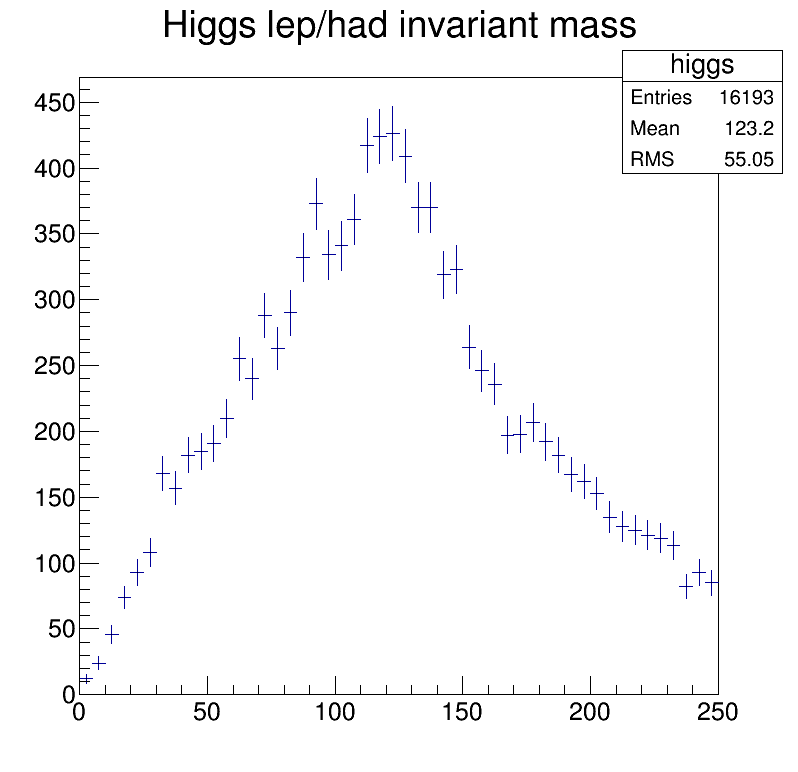
\includegraphics[scale=.36]{lep_had.png}
		 	%\caption{H boson mass for lep+had final state.}
		 \end{figure}
			 \begin{figure}[h]
			 	\centering
			 	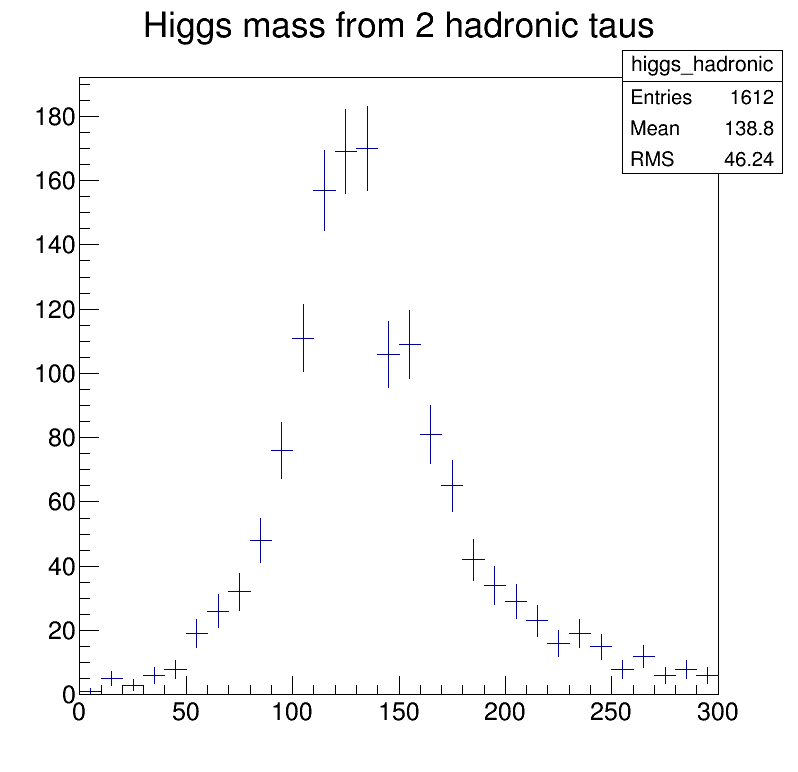
\includegraphics[scale=.31]{hadronic.png}
			 %	\caption{Leading b jets for hadronic final state}
			 \end{figure}
			  \begin{figure}[h]
			 	\centering
			 	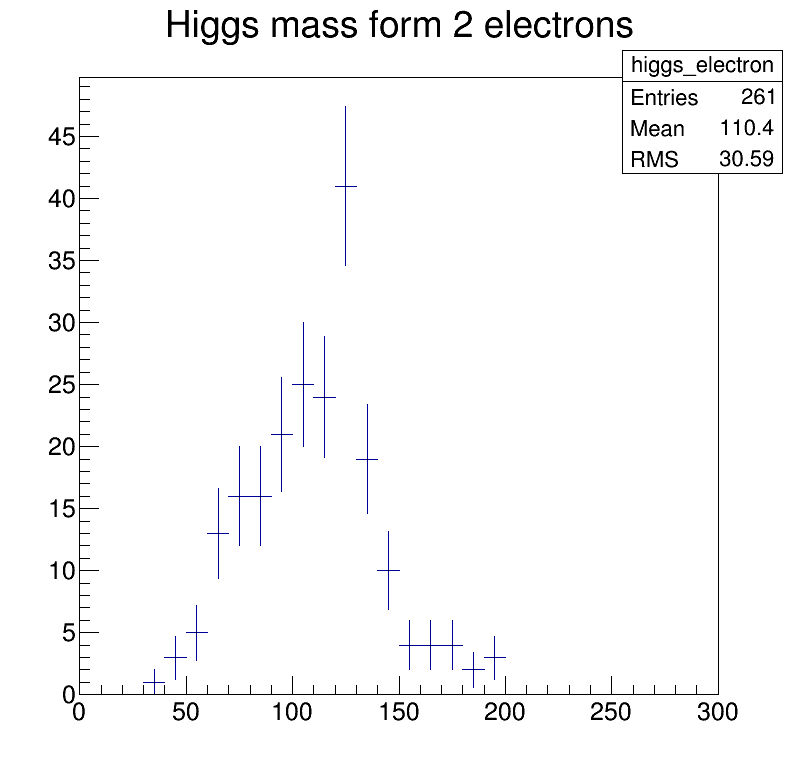
\includegraphics[scale=.31]{electronic.png}
			 %	\caption{Leading b jets for electron final state}
			 \end{figure}
			  \begin{figure}[h]
			 	\centering
			 	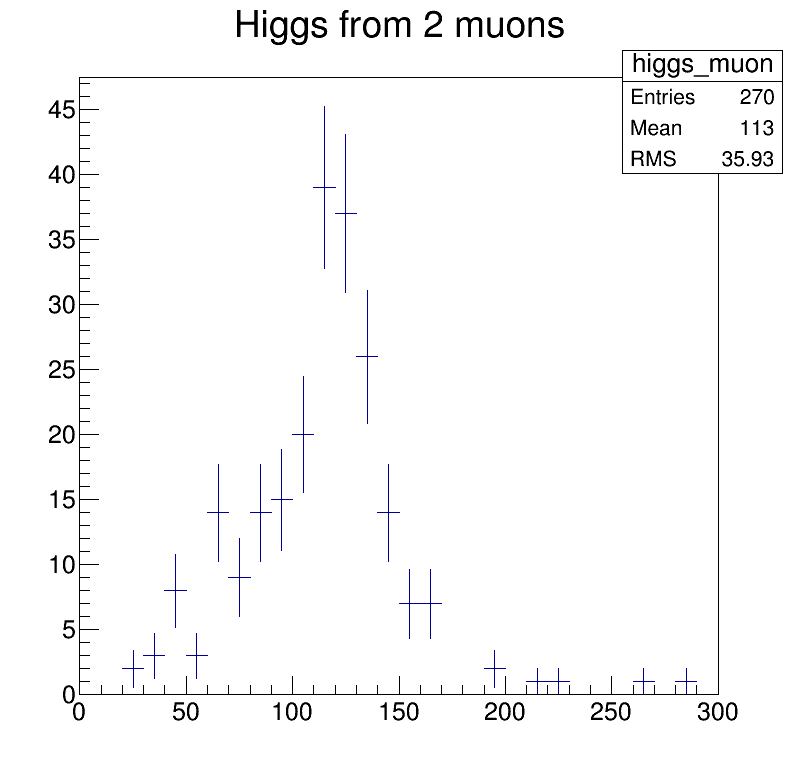
\includegraphics[scale=.31]{muonic.png}
			 %	\caption{Leading b jets for muonic final state}
			 \end{figure}
			  \begin{figure}[h]
			 	\centering
			 	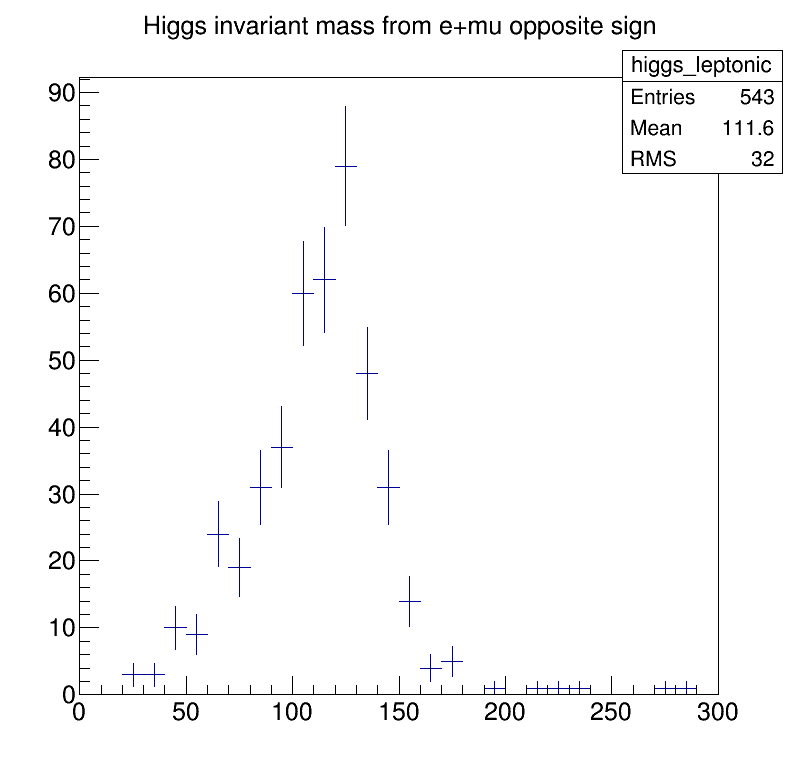
\includegraphics[scale=.31]{e+mu_op.png}
			 %	\caption{Leading b jets for e+mu opposite sign final state}
			 \end{figure}
			
	
\end{document}
This is never printed